\scanpage{57}

$F_0$ le Module qu'il induit sur $X_0$. On suppose a) Pour tout $s\quad S$,
la section $t_s$ induite par $t$ sur la fibre $X_s$ est
$\underline O_{X_s}$-régulière et $\underline F_s$-régulière
b) $\underline F$ et $\underline O_X$ sont plats par rapport à $S$
c) Pour tout $s\quad S$, $F_{0\,s}$, \deleted{et}
$\underline O_{X_{0\,s}}$ \inserted{et $\underline O_X$}
sont de profondeur $\quad 2$ en les points fermés de
$X_s\deleted{\unsure{s|z}}$.
Sous ces conditions, il existe un Module cohérent $F$ sur $X$, et un isomorphisme
de son complété formel $\hat F$ le long de $X_0$ avec $\underline F$.

Cet énoncé va résulter du suivant:

\uline{Corollaire} 3.2.\quad Sous les conditions de \unsure{3.1}.\quad (

\[
\coprod_{\substack{p\unsure{\gg|\ge}0\\q\geq0}}F_0(q-p)
\]
\[
M+M(1)+\cdots+M(-p)
\qquad
\coprod_{\unsure{0},q}S_q
\]

\figure{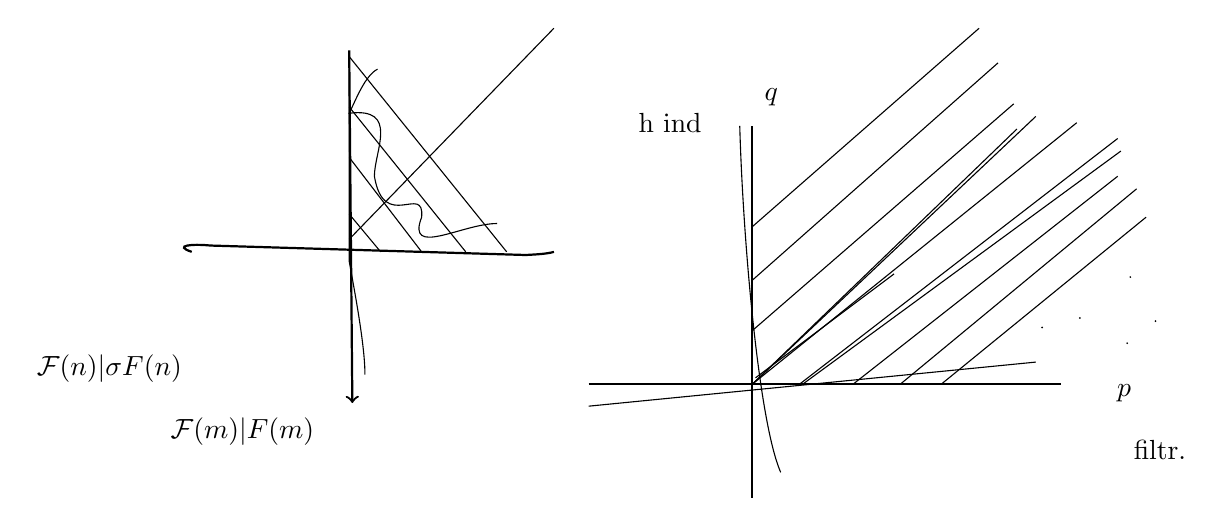
\begin{tikzpicture}[x=.8cm,y=.8cm]
\draw[thick] (-2.5,0) .. controls (-2.8,.1) and (-2.5,.13) .. (-2.2,.1)
 -- (2.8,-.05) .. controls (3,-.04) and (3.15,-.03) .. (3.25,0);
\draw[thick,->] (0,3.2) -- (.05,-2.4);
\draw[thin] (0,2.9) -- (0,-.15) .. controls (.1,-.7) and (.25,-1.5) .. (.25,-1.95);
\draw (0,3.1) -- (2.5,0);
\draw (0,2.3) -- (1.85,0);
\draw (0,1.5) -- (1.15,0);
\draw (0,.6) -- (.5,0);
\draw[thin] (0,.2) -- (3.25,3.55);
\draw[thin] (.45,2.9) .. controls (.25,2.8) and (.1,2.4) .. (0,2.2)
 .. controls (.8,2.3) and (.4,1.6) .. (.4,1.2)
 .. controls (.55,.3) and (1.2,1.1) .. (1.15,.55)
 .. controls (.9,-.1) and (1.8,.45) .. (2.35,.45);
\node[anchor=east] at (-2.5,-1.85) {$\unsure{\mathcal F(n)|\sigma F(n)}$};
\node[anchor=east] at (-.4,-2.85) {$\unsure{\mathcal F(m)|F(m)}$};
\begin{scope}[shift={(6.4,-2.1)}]
\draw[thick] (-2.6,0) -- (4.9,0);
\draw[thick] (0,-1.8) -- (0,4.1);
\draw[thin] (-.2,4.1) .. controls (-.15,2.3) and (.1,-.6) .. (.45,-1.4);
\draw[thin] (-2.6,-.35) -- (4.5,.35);
\draw (0,2.5) -- (3.6,5.65);
\draw (0,1.65) -- (3.9,5.1);
\draw (0,.85) -- (4.15,4.45);
\draw (0,0) -- (4.5,4.25);
\draw[thin] (0,0) -- (4.2,4.05);
\draw (0,0) -- (5.15,4.15);
\draw[thin] (.05,.1) -- (2.25,1.75);
\draw (.75,0) -- (5.8,3.9);
\draw[thin] (.8,0) -- (5.85,3.7);
\draw (1.6,0) -- (5.8,3.3);
\draw (2.35,0) -- (6.1,3.1);
\draw (3,0) -- (6.25,2.65);
\node at (.3,4.55) {$q$};
\node at (5.9,-.15) {$p$};
\node[anchor=east] at (-.65,4.15) {\unsure{h ind}};
\node[anchor=west] at (5.9,-1.05) {\unsure{filtr.}};
\fill (5.2,1.05) circle (.015);
\fill (6,1.7) circle (.015);
\fill (6.4,1) circle (.015);
\fill (5.95,.65) circle (.015);
\fill (4.6,.9) circle (.015);
\end{scope}
\end{tikzpicture}}

\diagram{\begin{tikzcd}
H^i(X,F)\arrow[r]&H^i(\hat X,\hat F)
\end{tikzcd}}

\margin{56}
